% !TEX ROOT=./main.tex



\section{Numerical Experiments}
\label{sec:exp}

In this section, we empirically examine the theoretical convergence rate of FedAvg on various scenarios, including strongly convex function, convex smooth function, and overparameterized setting, as presented in previous sections.

\textbf{Setup.} Follow the experimental setting in~\cite{stich2018local}, we
conduct experiments on both synthetic datasets and real-world dataset
w8a~\cite{platt1998fast} $(d=300, n=49749)$. We consider the distributed
objectives $F(\vw) = \sum_{k=1}^N p_kF_k(\vw)$, and the objective function on
each local device $k$ includes three cases: 1) \textbf{Strongly convex
objective}: the regularized binary logistic regression problem, $F_k(\vw) =
\frac{1}{N_k} \sum_{i=1}^{N_k} \log( 1+ \exp(-y_i^k \vw^T\vx_i^k) + \lambda
\|\vw\|^2$. The regularization parameter is set to $\lambda = 1/n \approx
1e-5$. 2) \textbf{Convex smooth objective}: the binary logistic regression
problem without regularization. $F_k(\vw) = \frac{1}{N_k} \sum_{i=1}^{N_k}
\log( 1+ \exp(-y_i^k \vw^T\vx_i^k)$. 3) \textbf{Overparameterized setting}:
the linear regression problem without adding noise to the label, $F_k(\vw) =
\frac{1}{N_k} \sum_{i=1}^{N_k} (\vw^T\vx_i^k + b  - y_i^k)^2$.  In the first
two cases, we use the w8a dataset to conduct empirical evaluation. 
In the linear regression problem, we use features from w8a dataset and 
generate a ground truth $w$ to label each instance, which satisfies the
overparameterized setting. For the detailed experimental setup and
hyperparameter setting, please refer to the section~\ref{sec:expsupp} in the
appendix.


% ~\ref{th:strongcvxsmth}~\ref{th:cvxsmoth}~\ref{th:fedmasslr}
\textbf{Linear speedup.} To verify the linear speedup results in Theorems
\lkxcom{cite sgd theorems}, we evaluate the number of iterations needed to reach
$\epsilon$-accuracy in three objectives. We initialize all runs with $\vw_0 = \textbf{0}_d$ and measure. For each configuration, we run three random seeds and report
the best seed results for each configuration $(E, K)$. In each configure, we
extensive search the stepsize from $\min(\eta_0, \frac{nc}{1 + t})$, where
$\eta_0 \in \{0.1, 0.12, 1, 32 \}$ according to different problems and $c$ can
take the values $c = 2^i \ \forall i \in \ZZ$. As the results shown in Figure~\ref{fig:speedup},
the number of iterations to reach the target accuracy $\epsilon$ decreasing 
as the number of workers increase. 

\textbf{The impact of $E$.} We further examine how does the number of epochs 
affect the convergence. As shown in Figure~\ref{fig:e}, the number of iterations
increases as the number of epochs increase, which slow the convergence in
terms of gradient computation. However, it can save communication cost as
the number of rounds decreased when the number of epochs increases.


\textbf{Partial participations.} We verify the linear speedup in the
partial participation settings, where we set $50\%$ of devices
are active. As the results shown in Figure~\ref{fig:partial}, the 
FedAve enjoys linear speedup in various settings even with partial
device participation.

\textbf{Nesterov accelerated FedAvg.} In Figure~\ref{fig:nesterov}, 
report the convergence of Nesterov accelerated FedAvg. The empirical 
observation is aligned with our theorems \lkxcom{cite accelerated theorems} that the acclerated version of FedAvg can also achieve the lienar speedup
w.r.t the number of nodes.

\begin{figure}
\centering
	\begin{tabular}{ccc}
	\hspace{-2em}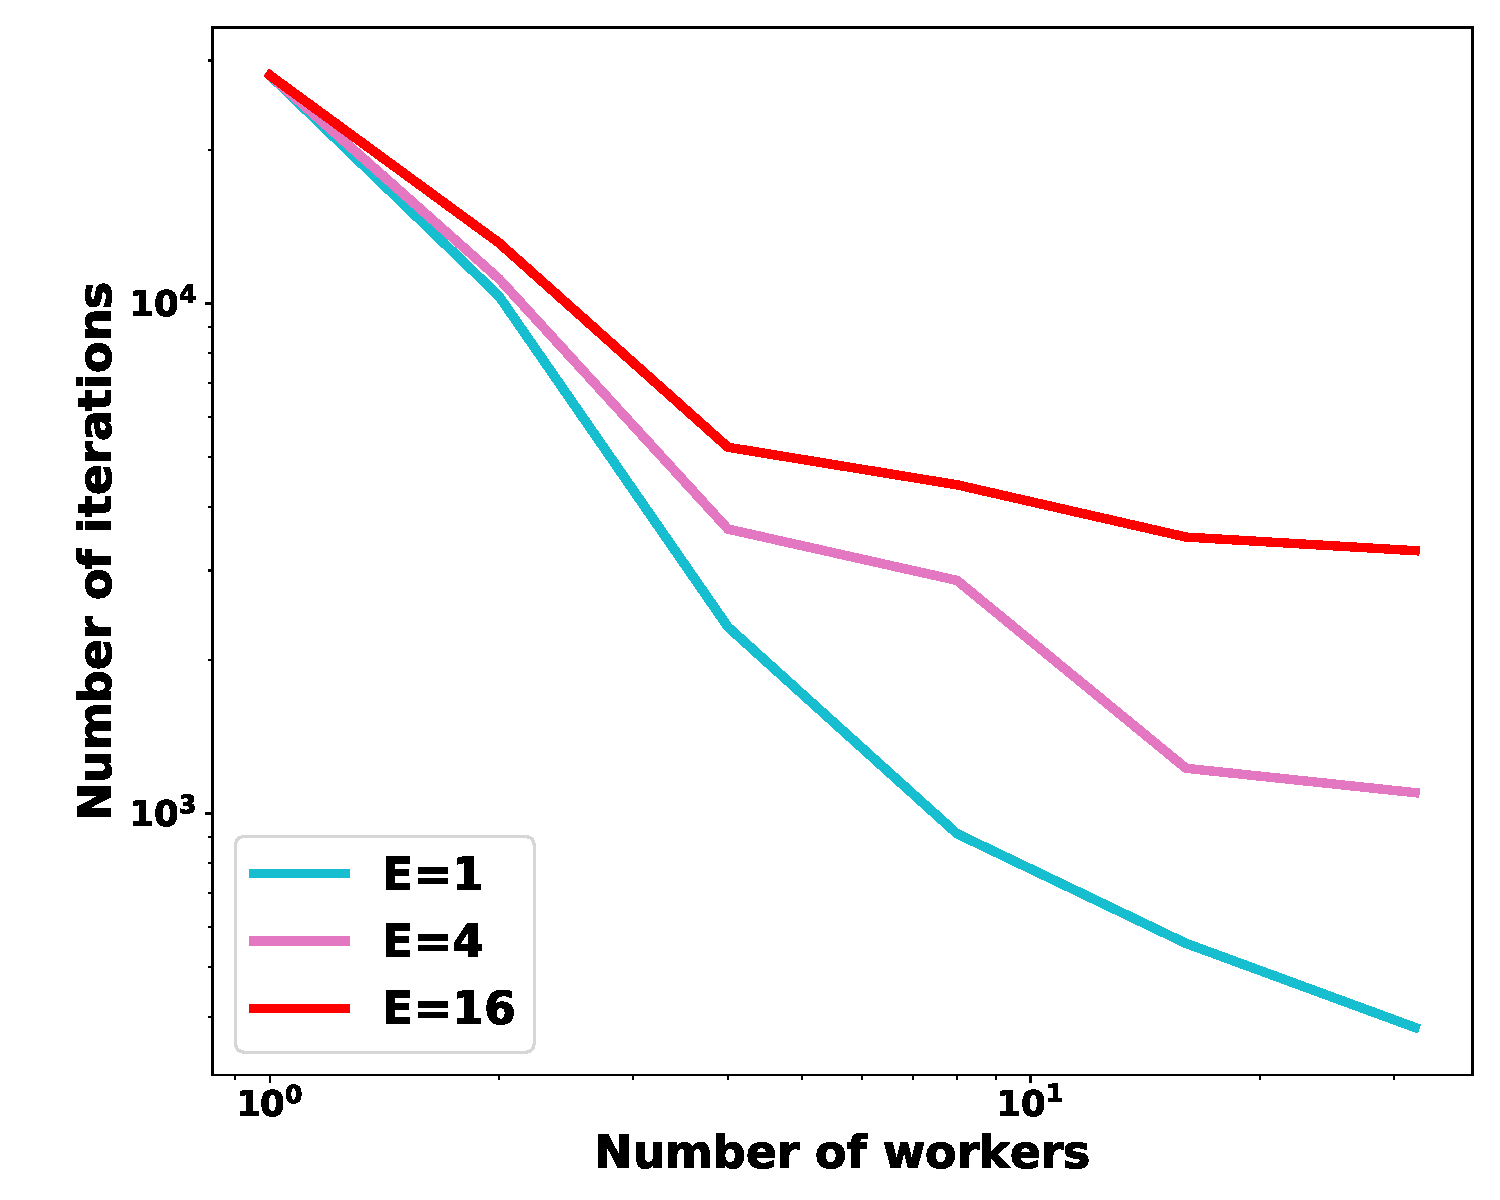
\includegraphics[width=0.33\textwidth]{fig/paper-stronglycvxsmthspeedupNodesT-min-w8a-epsilon0131-reg1e-05.pdf} &
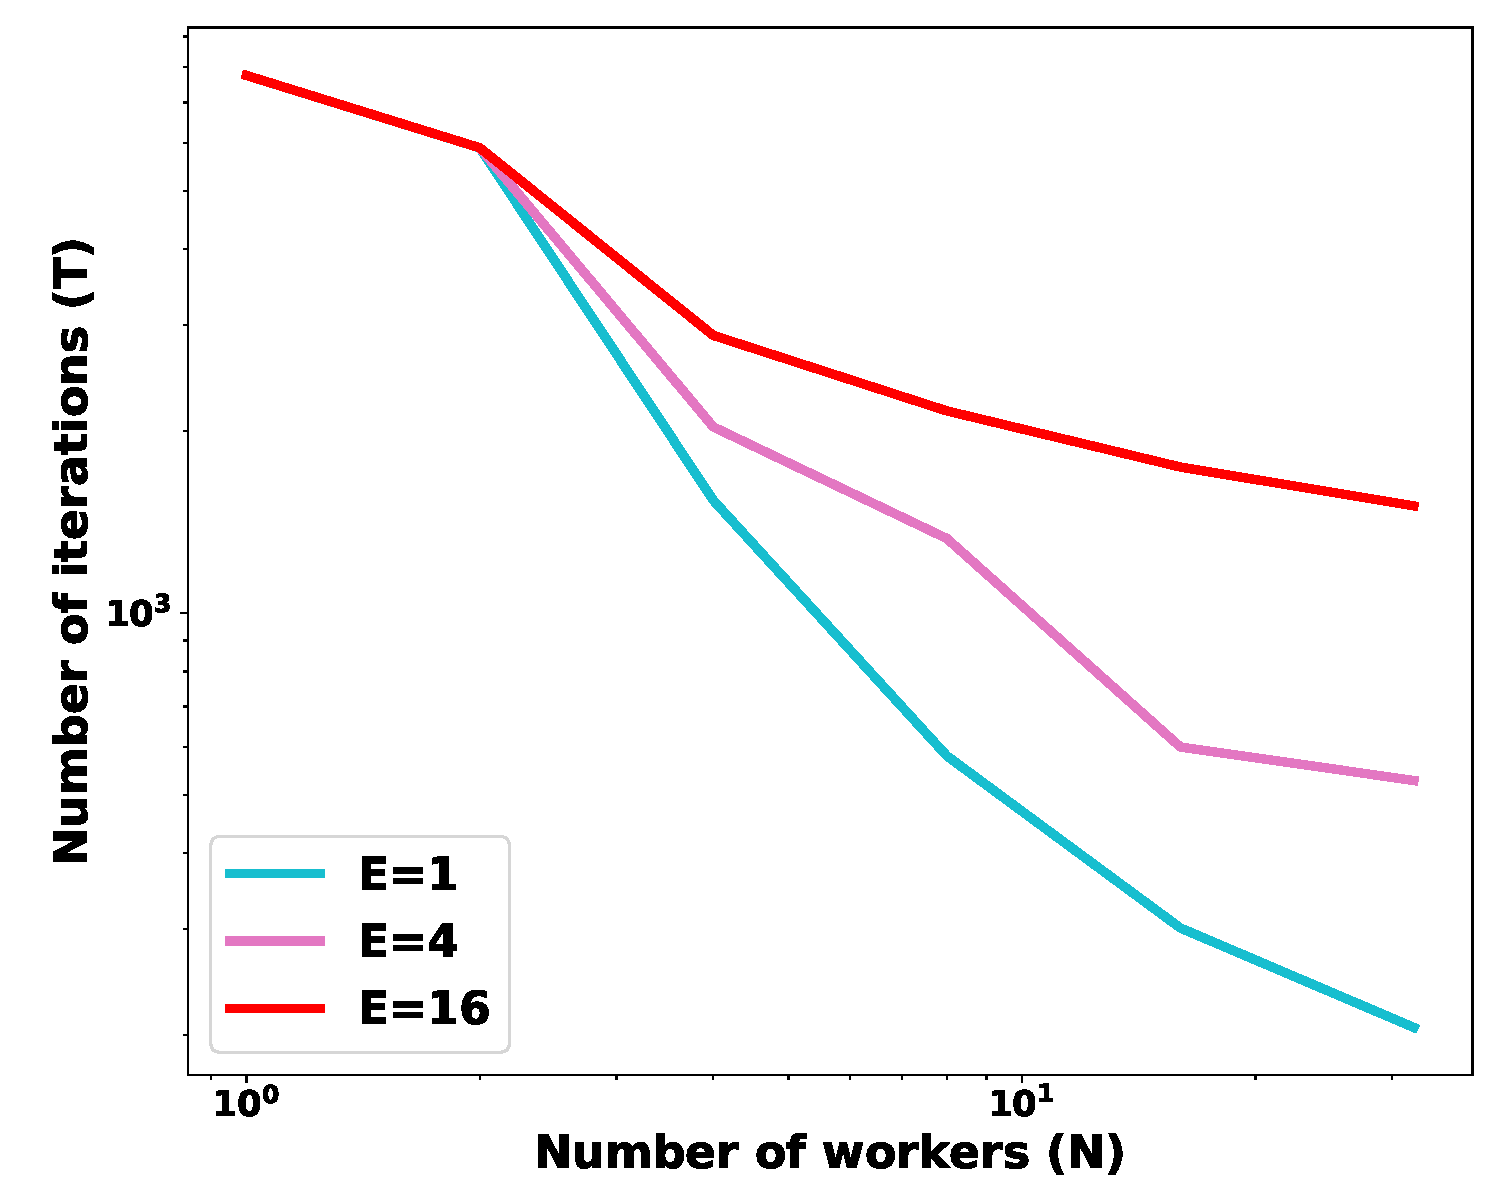
\includegraphics[width=0.33\textwidth]{fig/paper-cvxsmoothspeedupNodesT-min-w8a-epsilon0134-reg0.pdf} &
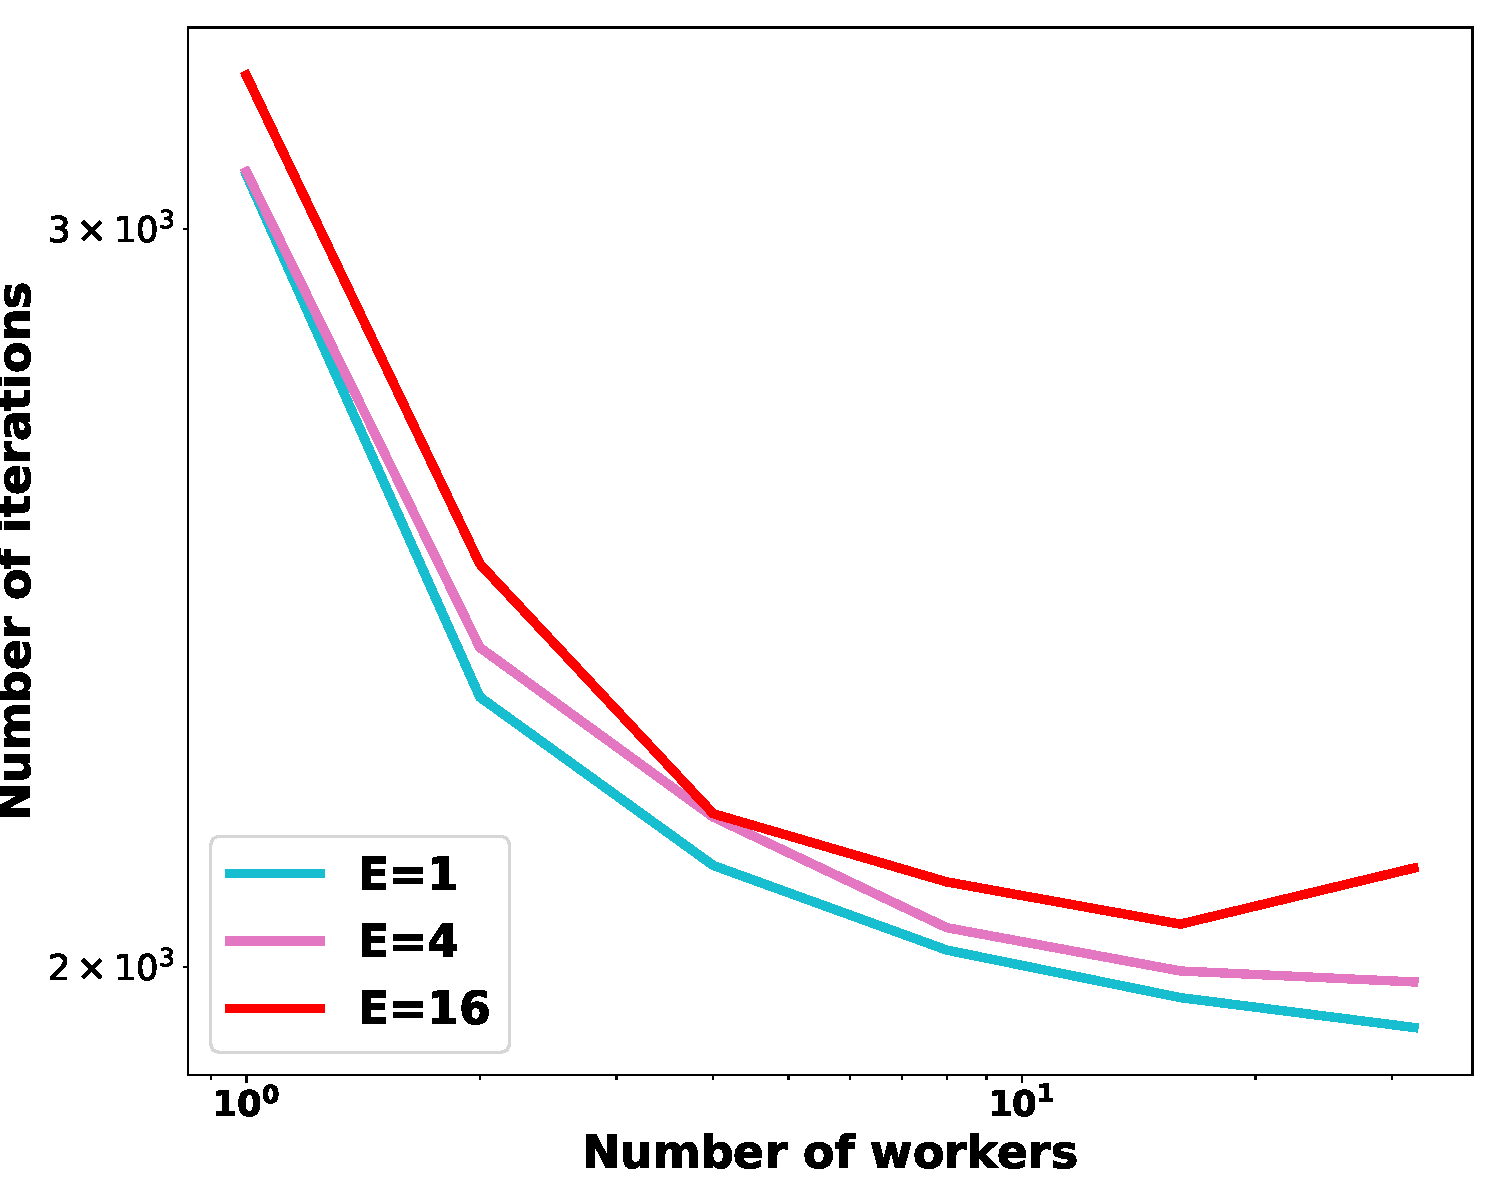
\includegraphics[width=0.33\textwidth]{fig/paper-linregressionspeedupNodesT-min-linearregressionw8a-epsilon002-reg0.pdf}\\
(a) Strongly convex objective & (b) Convex smooth objective & (c) Linear regression
	\end{tabular}
\caption{The linear speedup convergence of FedAvg w.r.t the number of workers. }
\label{fig:speedup}
\end{figure}

\begin{figure}
\centering
	\begin{tabular}{ccc}
	\hspace{-2em} 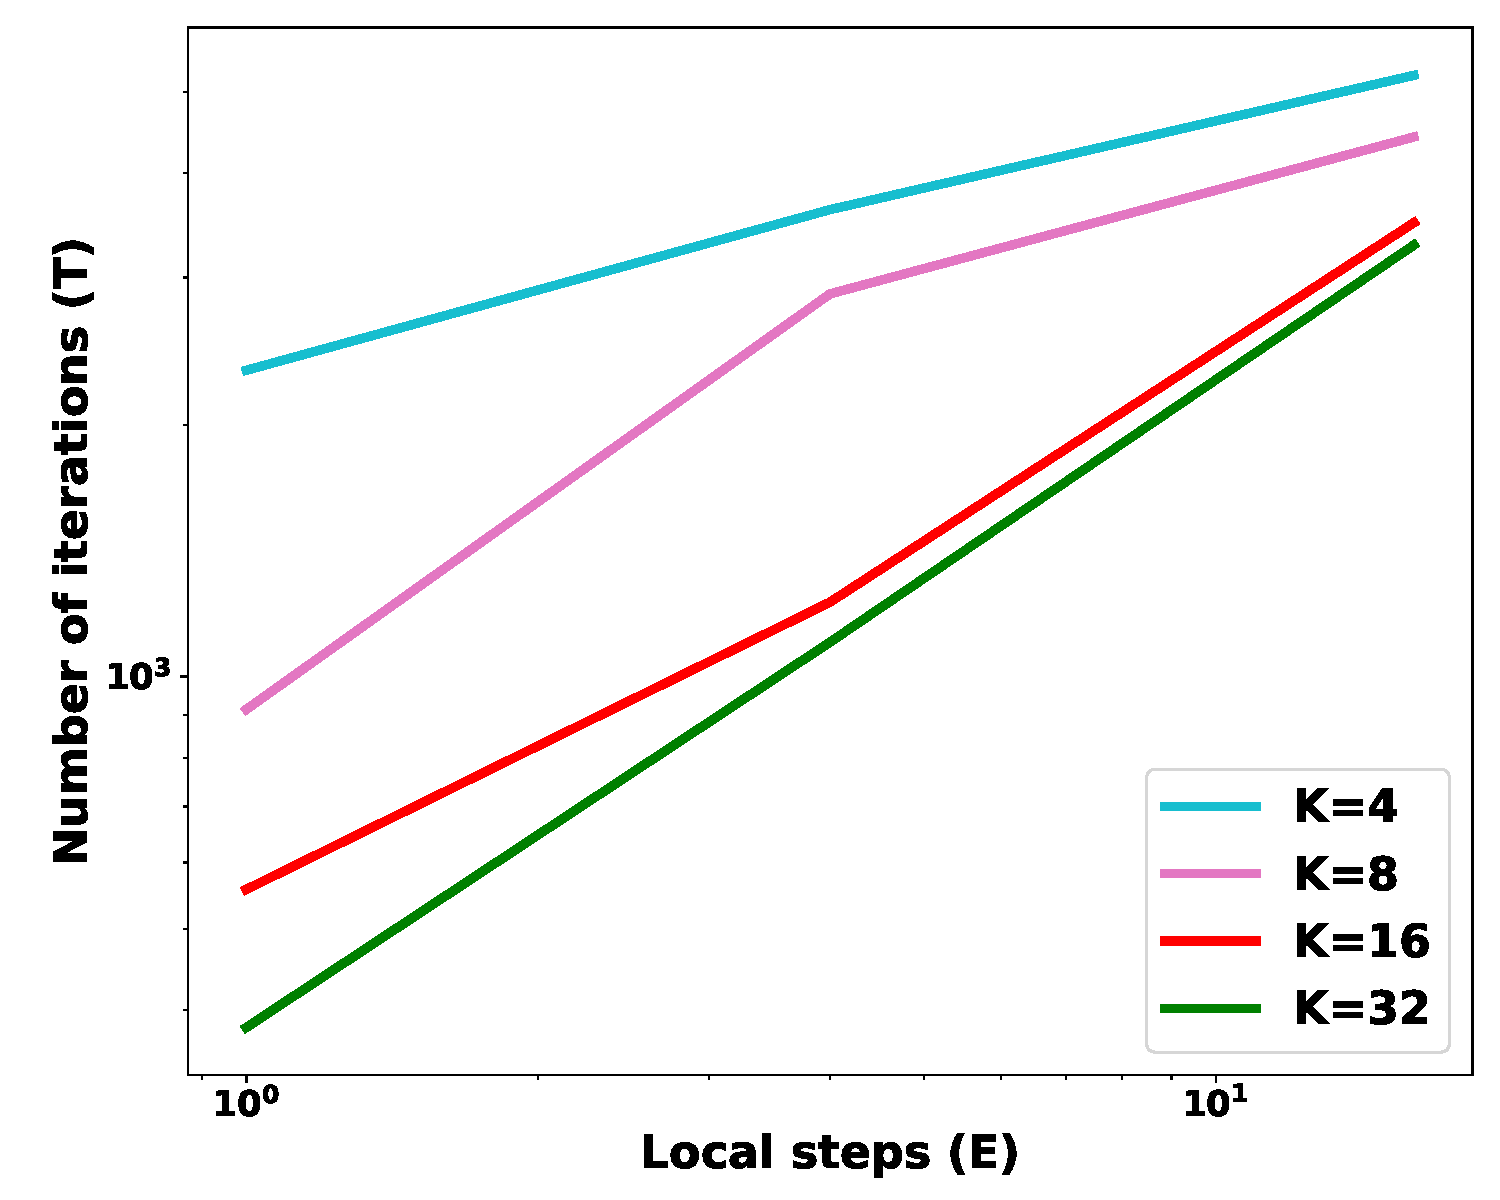
\includegraphics[width=0.33\textwidth]{fig/paper-stronglycvxsmthspeedupEpochsT-min-w8a-epsilon0131-reg1e-05.pdf} &
	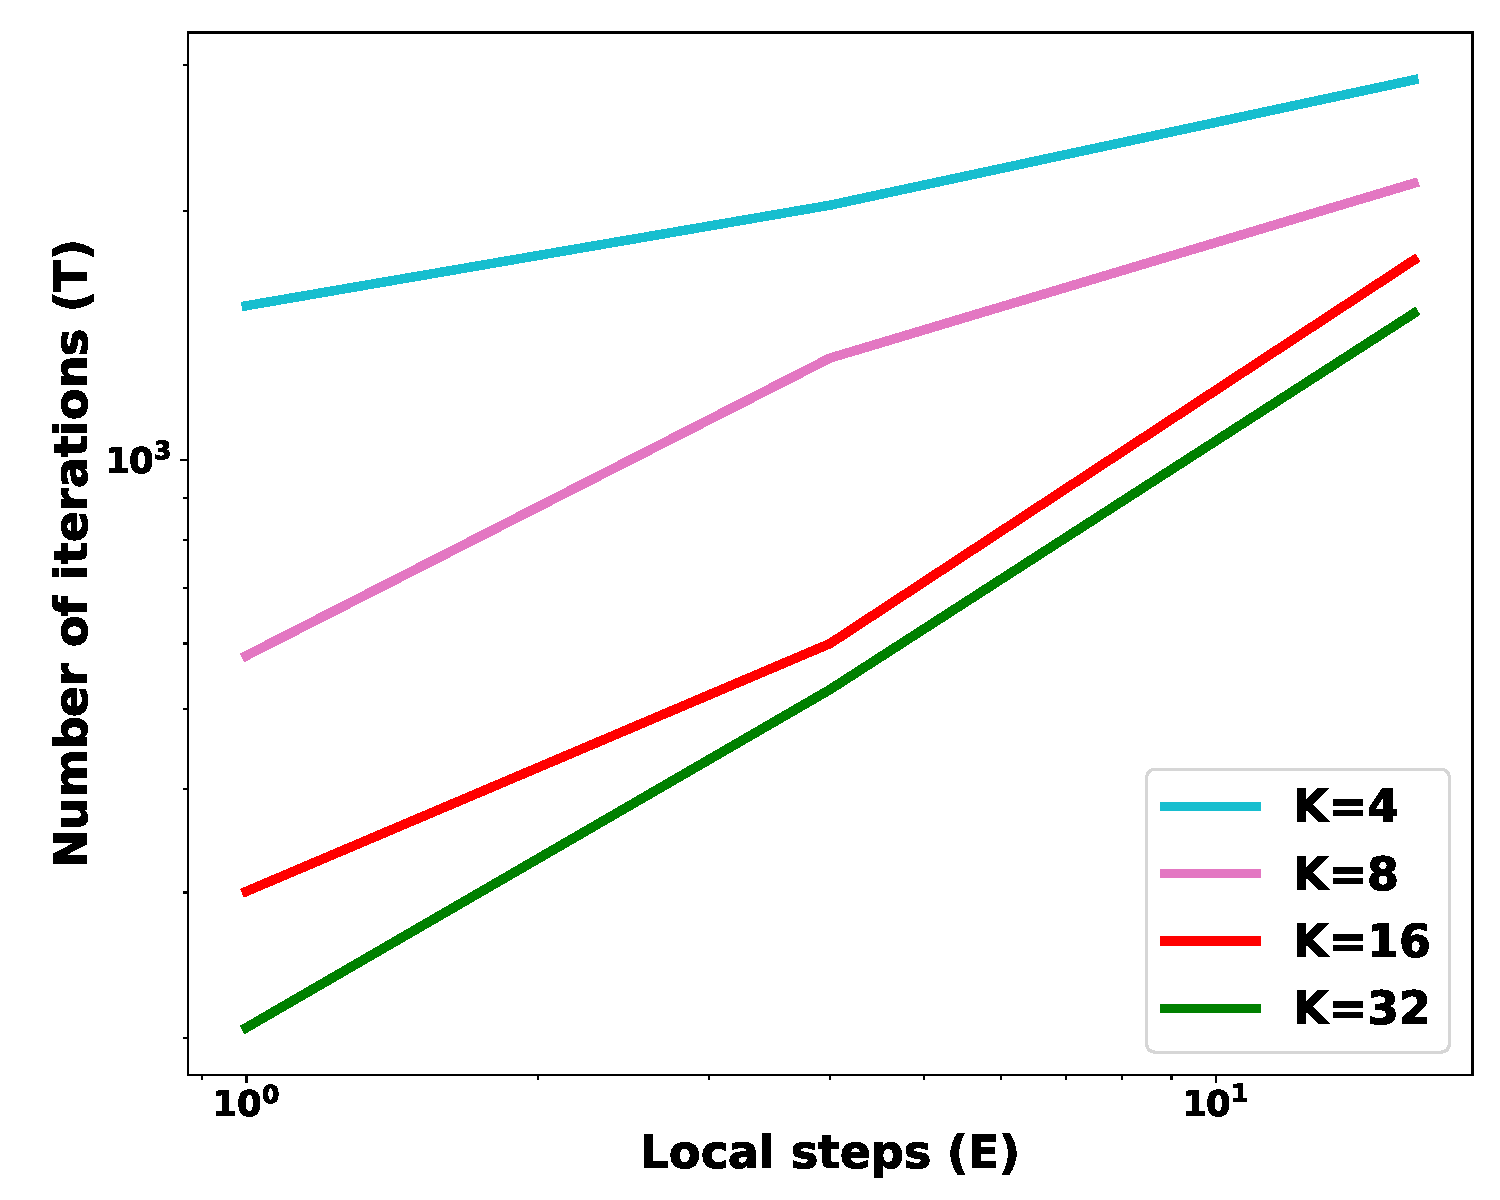
\includegraphics[width=0.33\textwidth]{fig/paper-cvxsmoothspeedupEpochsT-min-w8a-epsilon0134-reg0.pdf} & 
	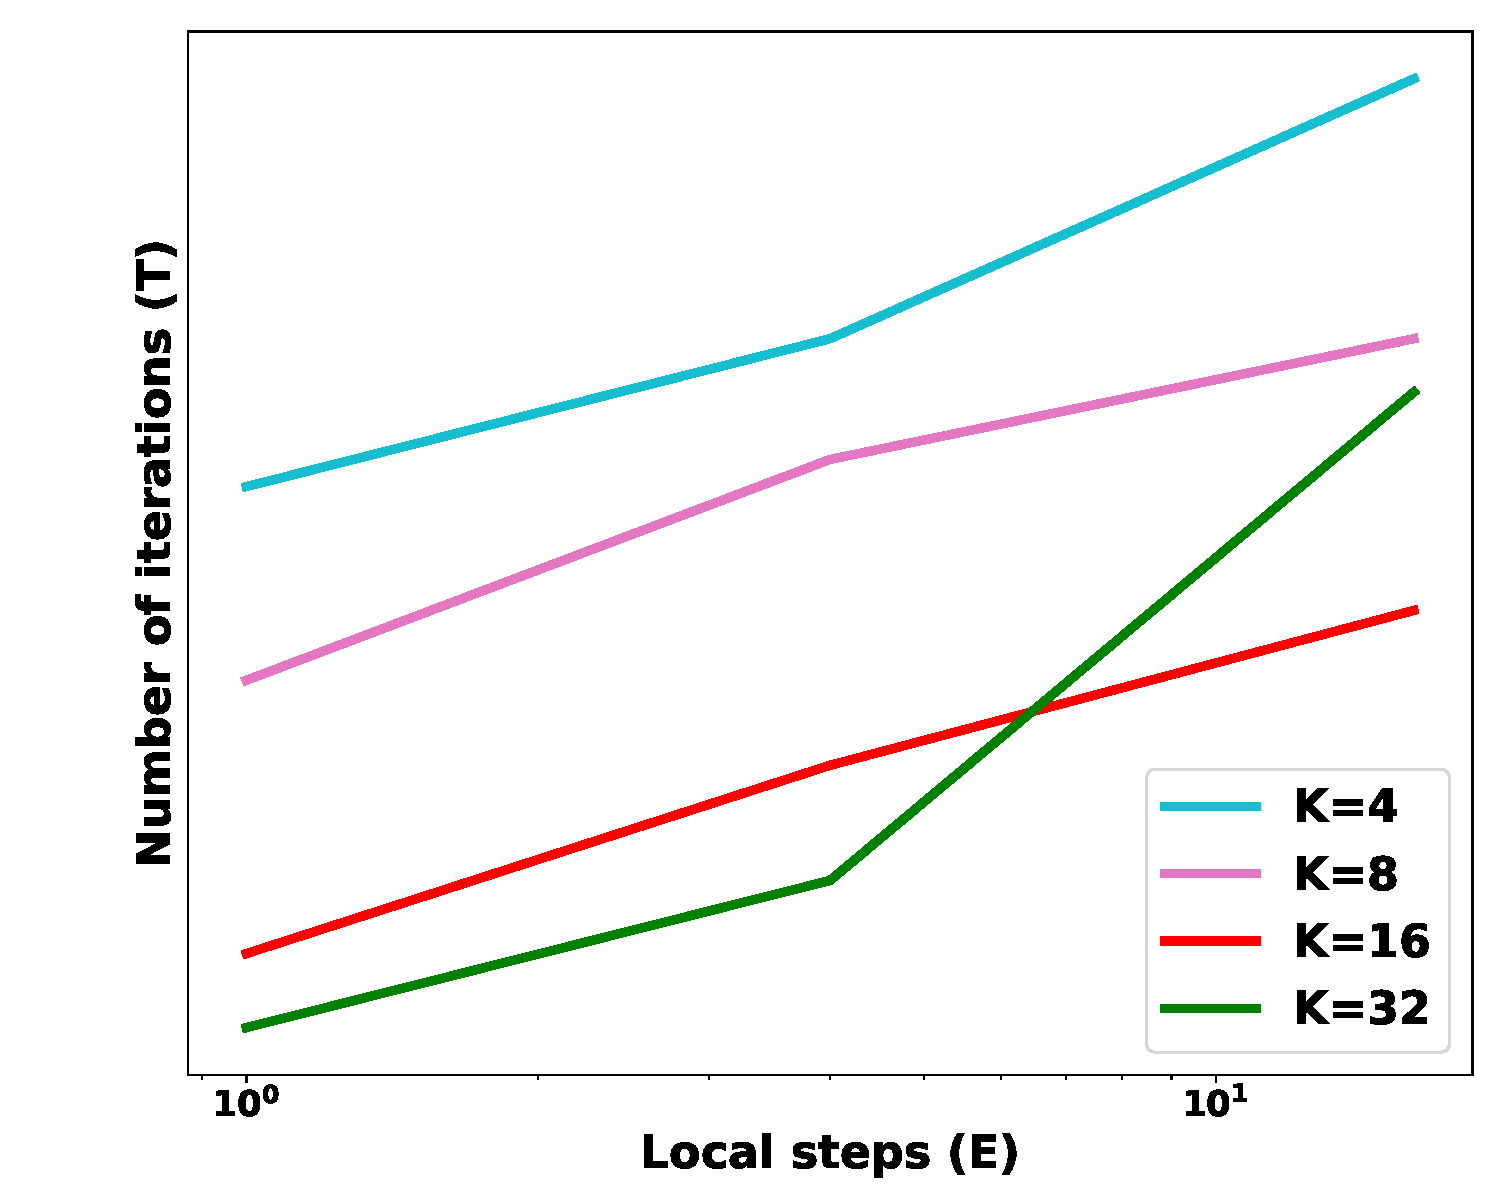
\includegraphics[width=0.33\textwidth]{fig/paper-linregression-newspeedupEpochsT-min-linearregressionw8a-epsilon002-reg0.pdf} \\
	\hspace{-2em} 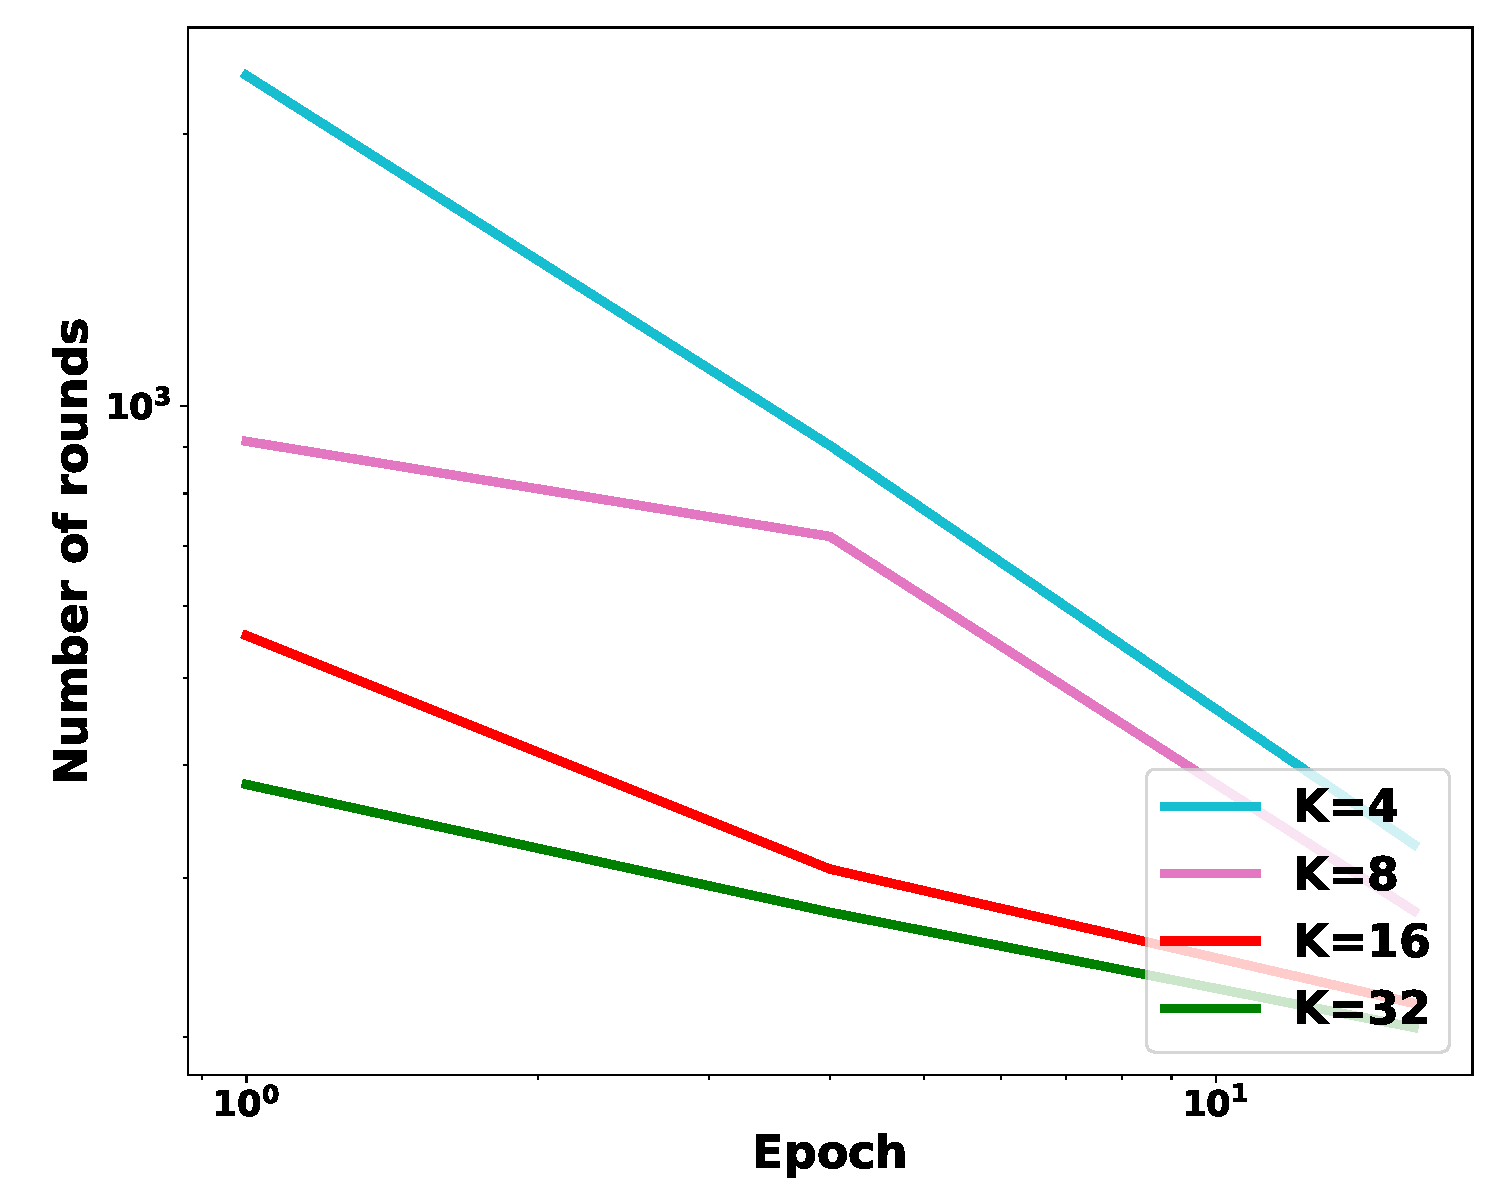
\includegraphics[width=0.33\textwidth]{fig/paper-stronglycvxsmthspeedupEpochsRounds-min-w8a-epsilon0131-reg1e-05.pdf} &
	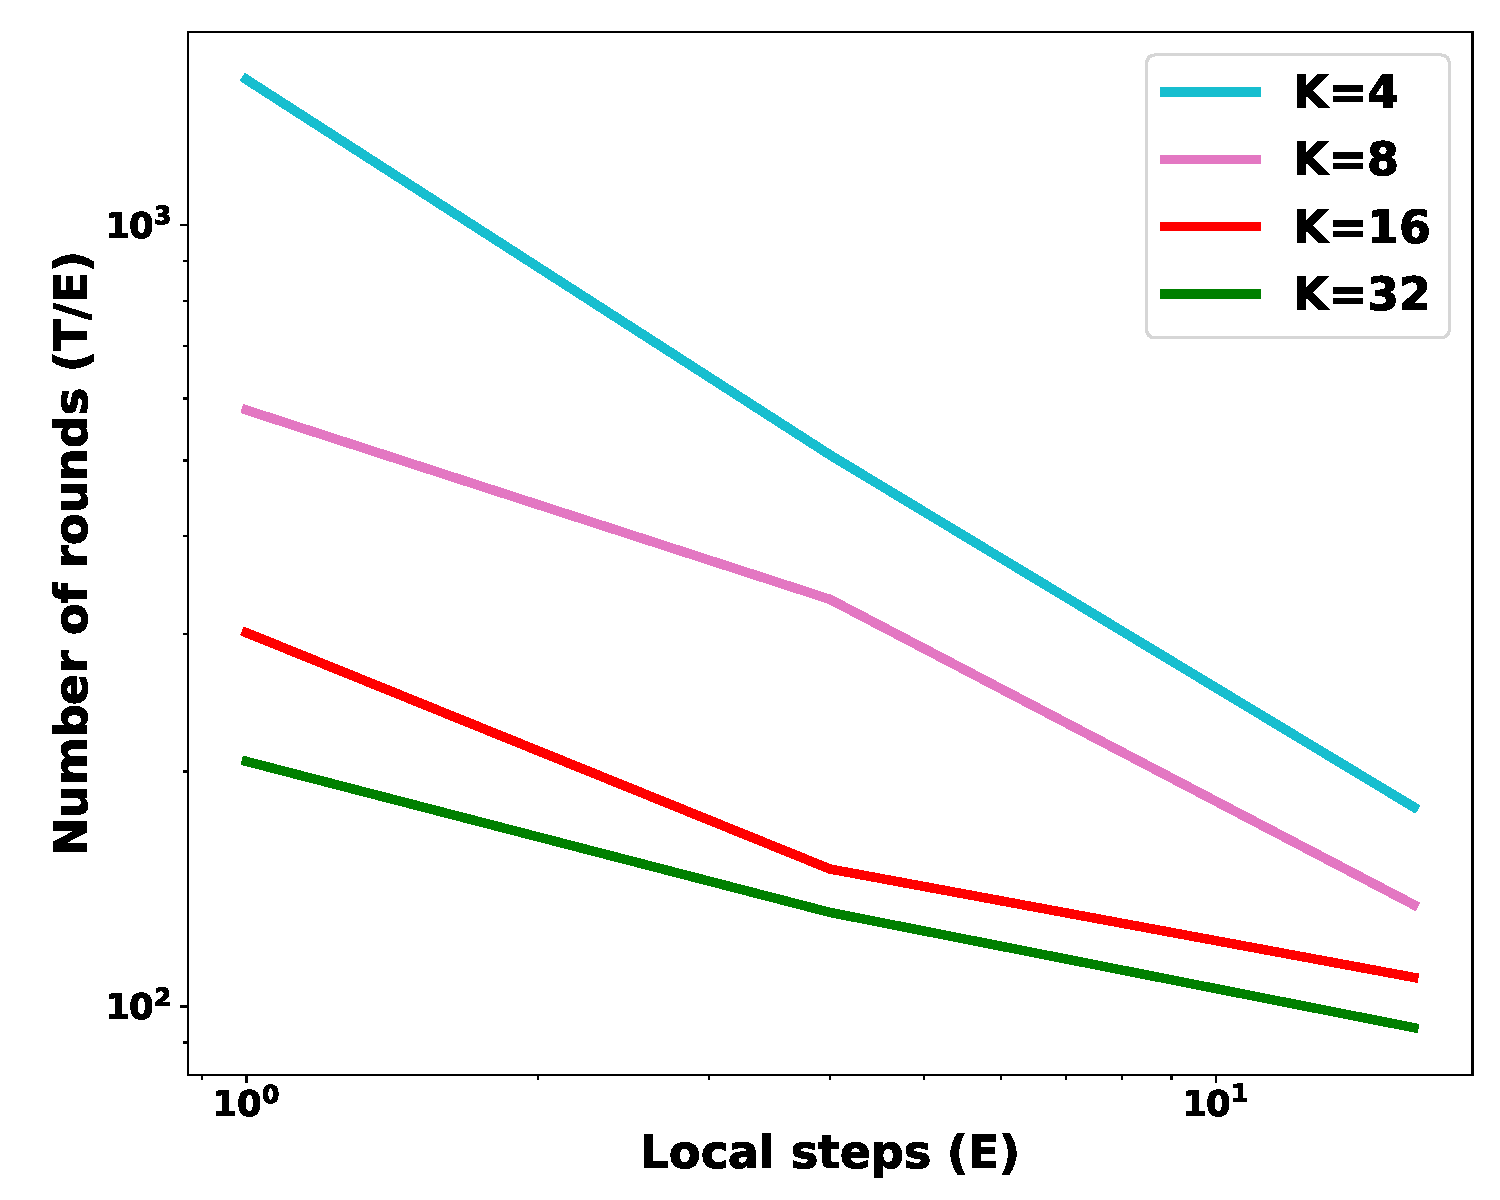
\includegraphics[width=0.33\textwidth]{fig/paper-cvxsmoothspeedupEpochsRounds-min-w8a-epsilon0134-reg0.pdf} & 
	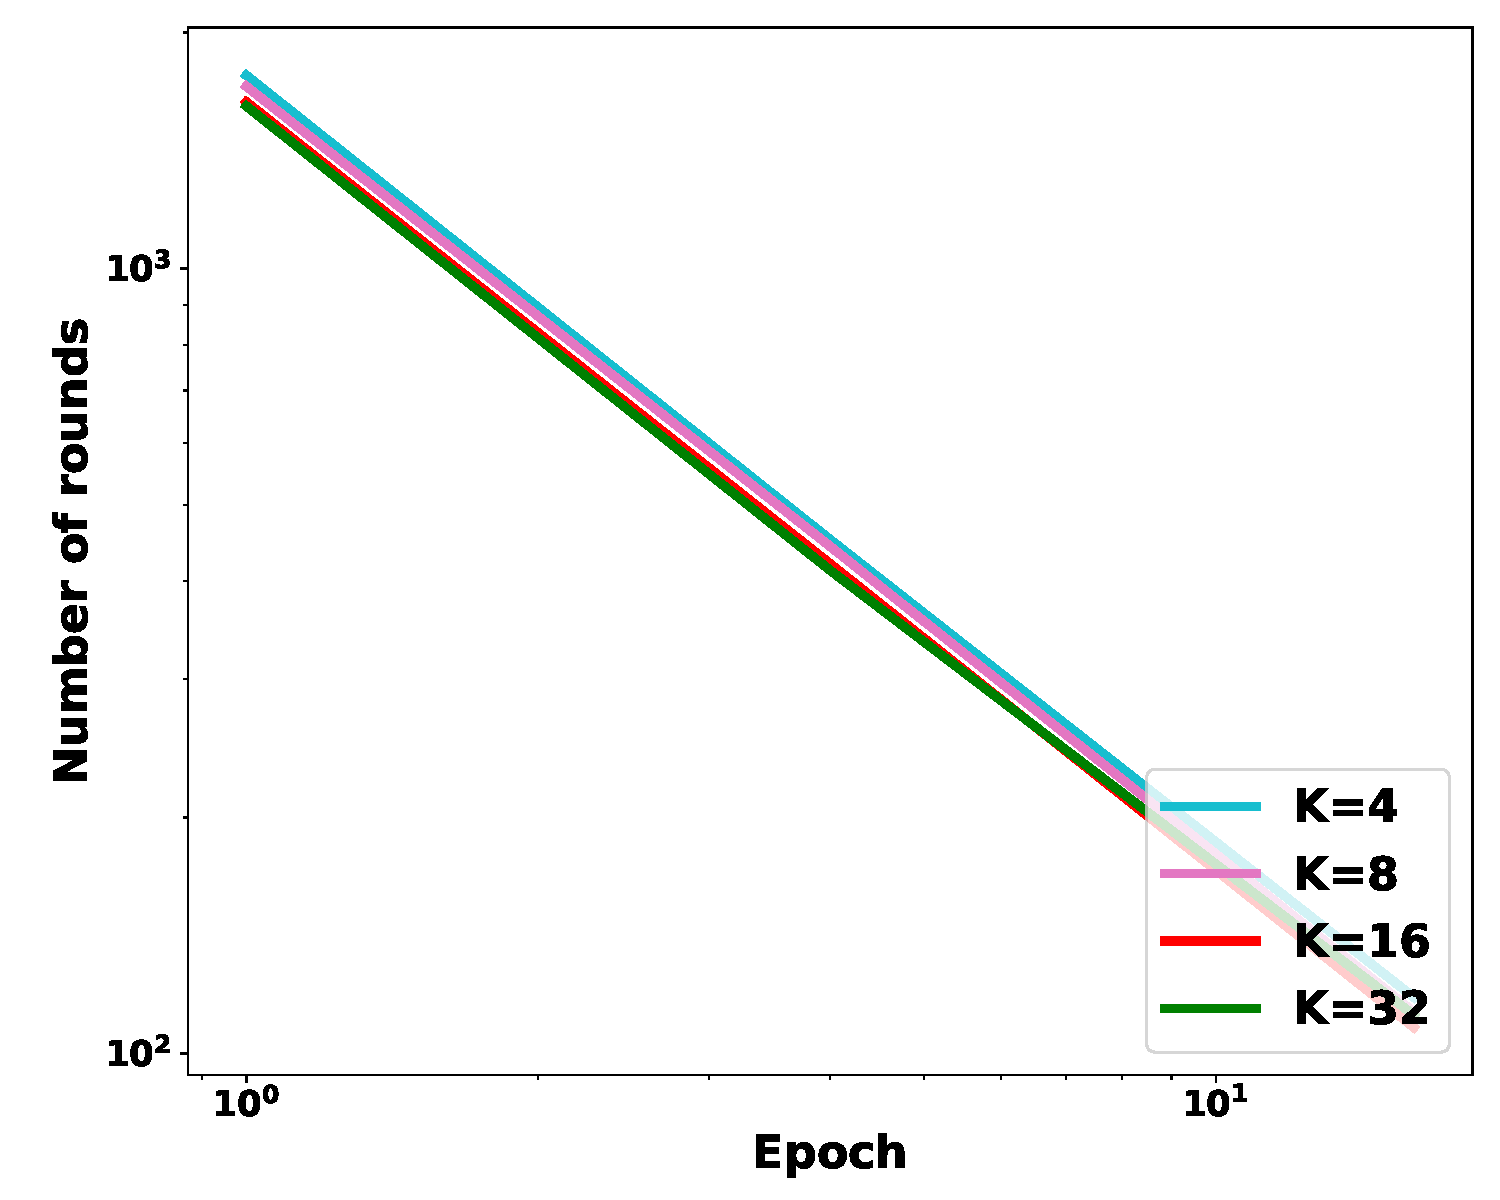
\includegraphics[width=0.33\textwidth]{fig/paper-linregression-newspeedupEpochsRounds-min-linearregressionw8a-epsilon002-reg0.pdf} \\
(a) Strongly convex objective & (b) Convex smooth objective & (c) Linear regression
	\end{tabular}
\caption{The convergence of FedAvg w.r.t the number of epochs. }
\label{fig:e}
\end{figure}

\begin{figure}
\centering
	\begin{tabular}{ccc}
	\hspace{-2em}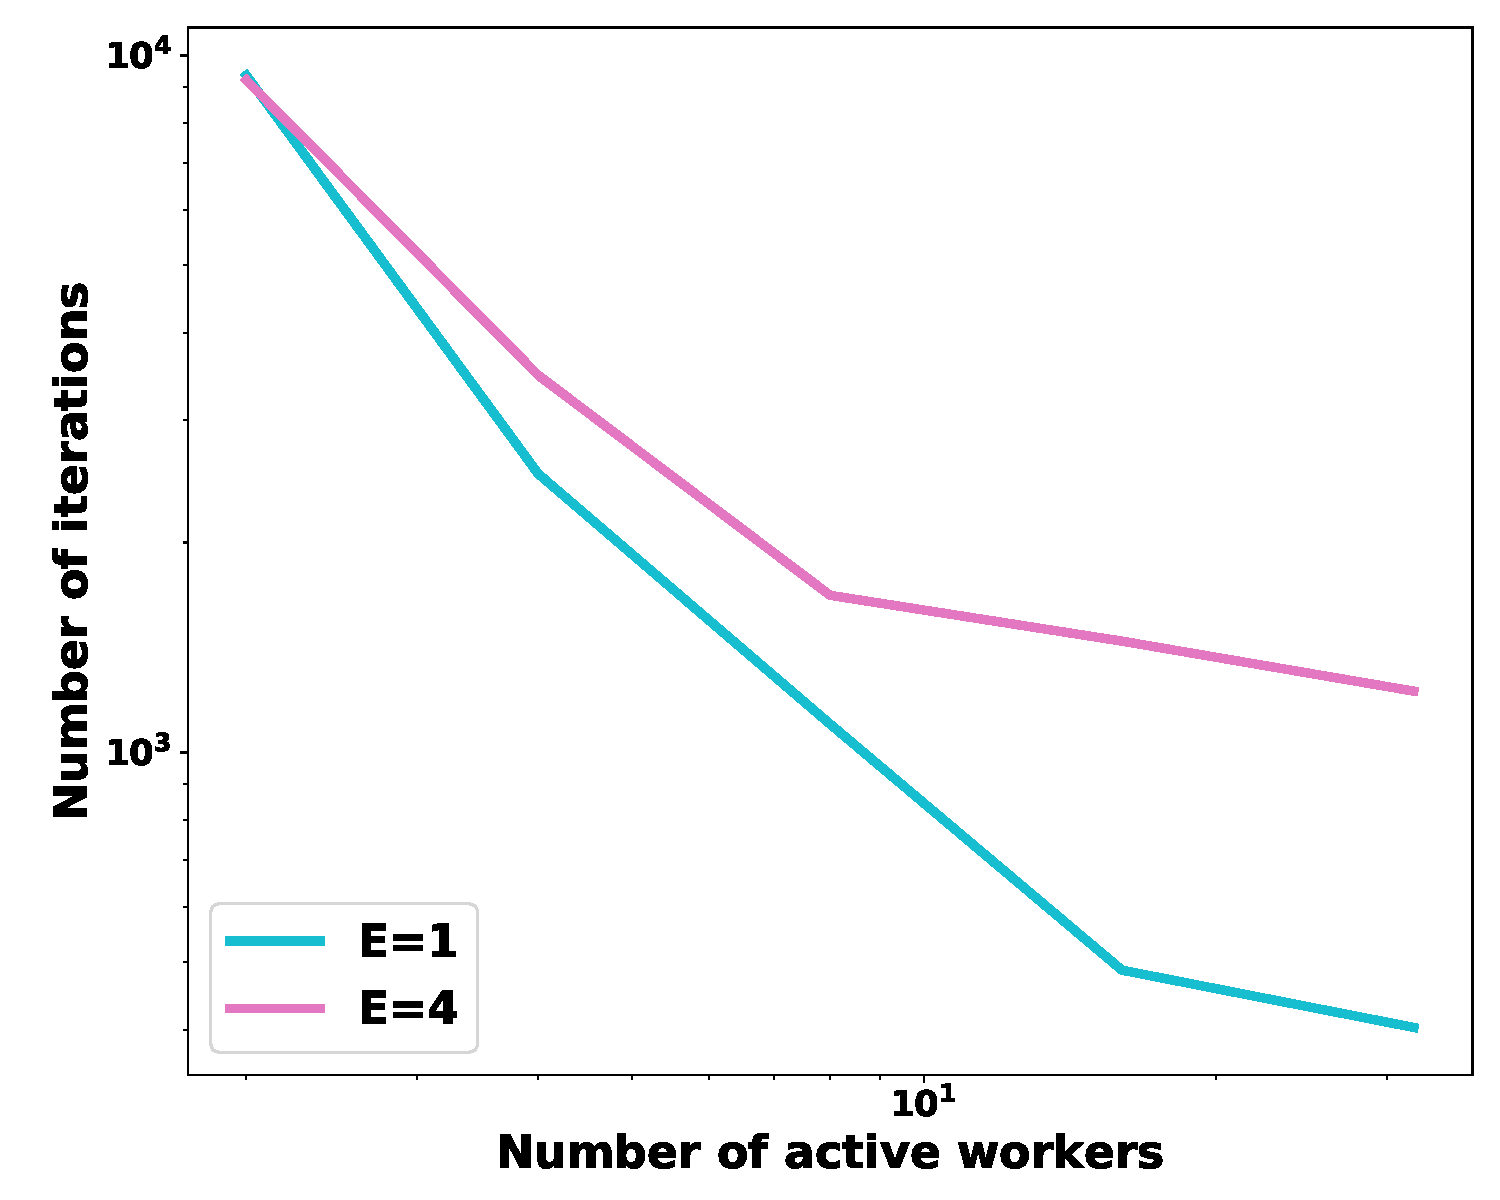
\includegraphics[width=0.33\textwidth]{fig/paper-partialstronglycvxsmthspeedupNodesT-min-w8a-epsilon0131-reg1e-05.pdf} &
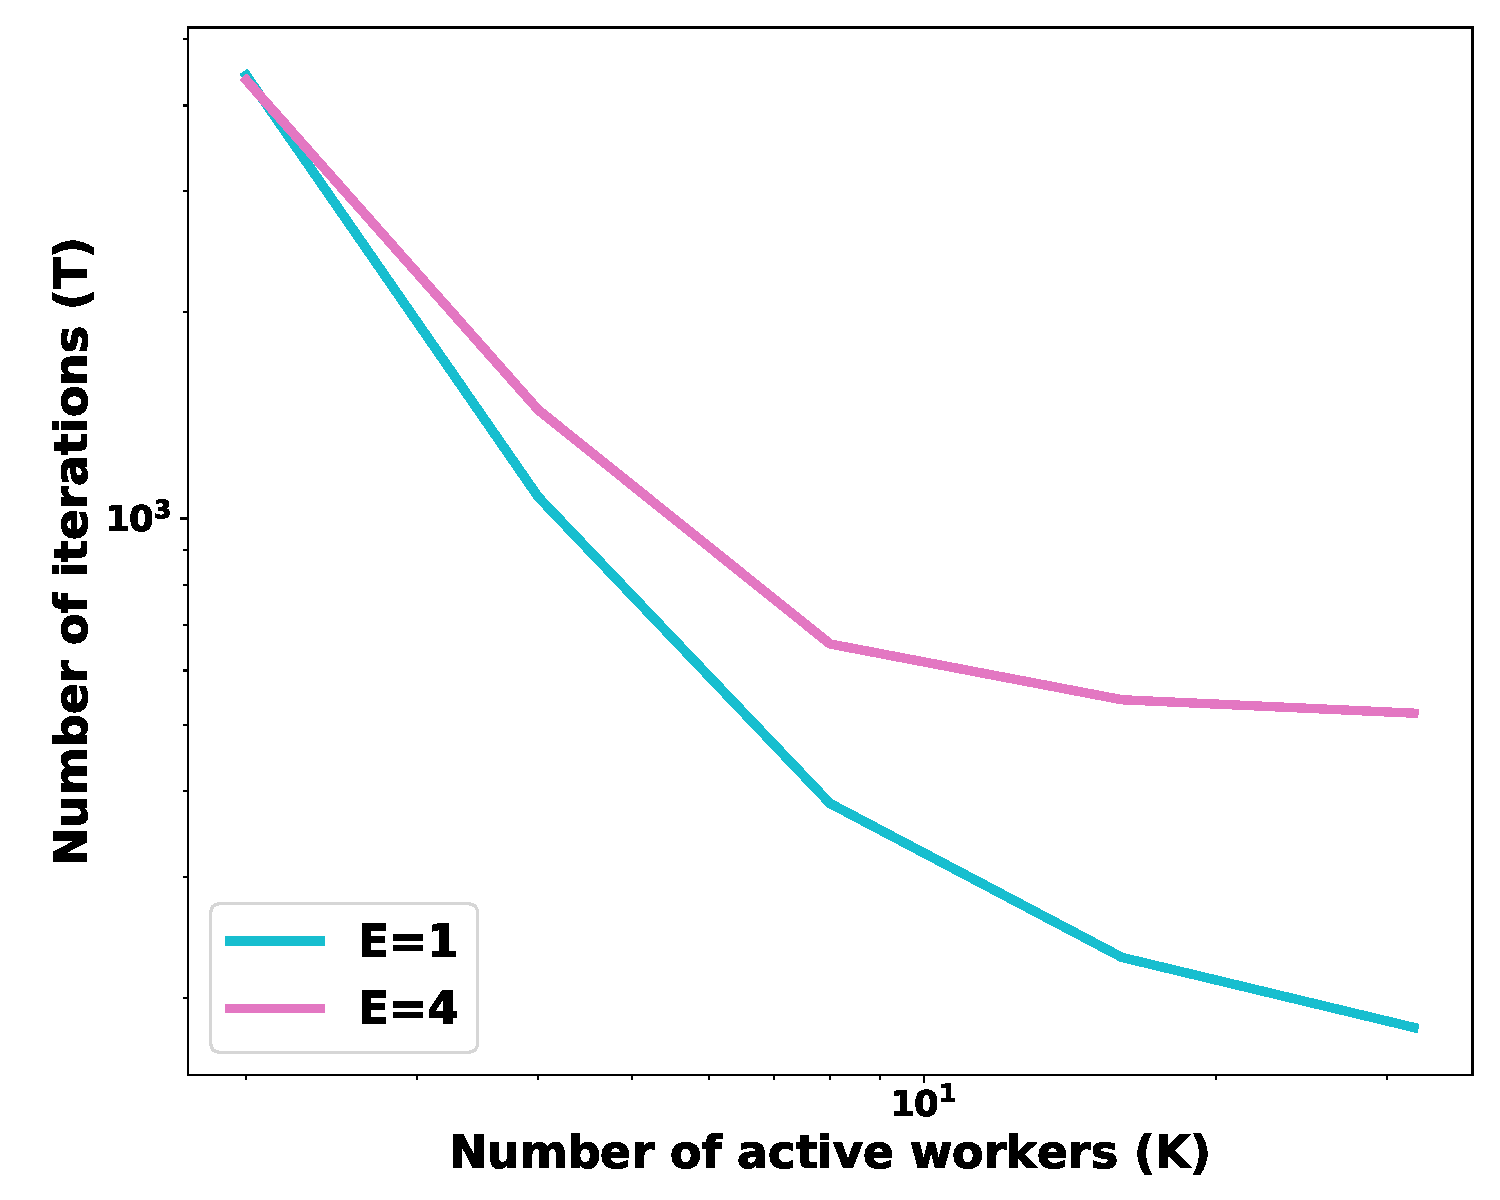
\includegraphics[width=0.33\textwidth]{fig/paper-partialcvxsmoothspeedupNodesT-min-w8a-epsilon0134-reg0.pdf} &
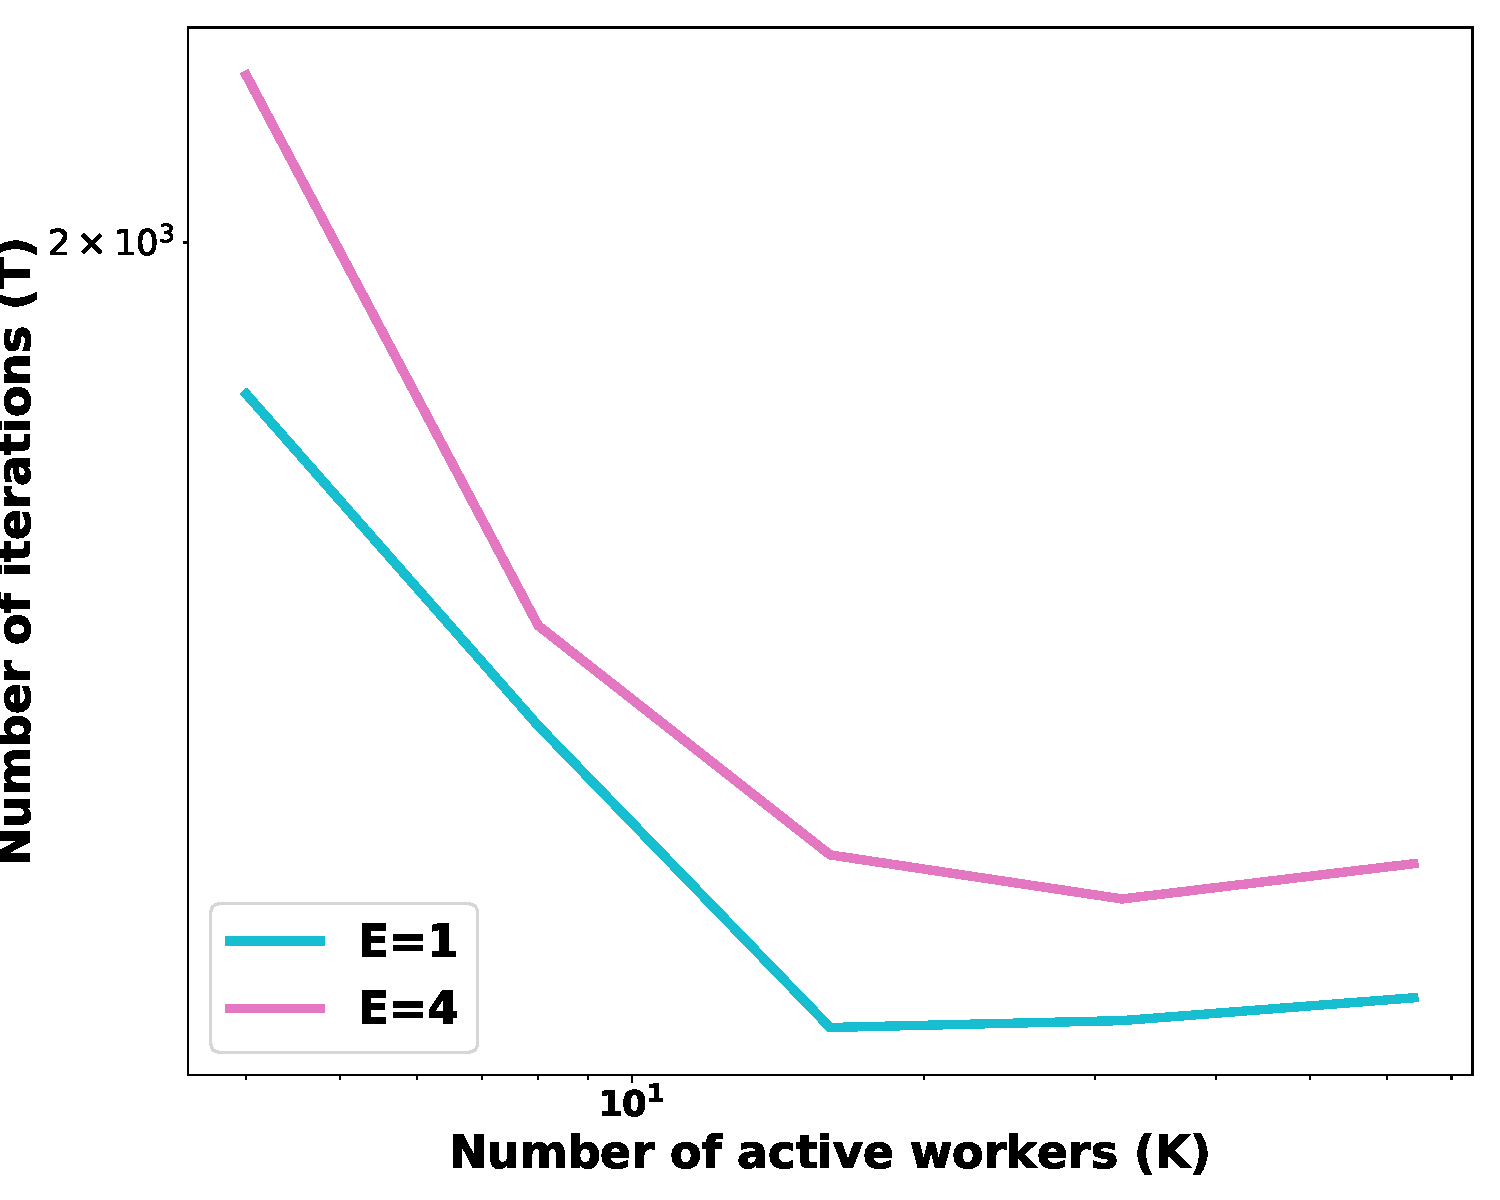
\includegraphics[width=0.33\textwidth]{fig/paper-partiallinregressionspeedupNodesT-min-linearregressionw8a-epsilon002-reg0.pdf}\\
(a) Strongly convex objective & (b) Convex smooth objective & (c) Linear regression
	\end{tabular}
\caption{The linear speedup convergence of FedAvg w.r.t the number of active workers. }
\label{fig:partial}
\end{figure}


\begin{figure}
\centering
\begin{tabular}{ccc}
\hspace{-2em}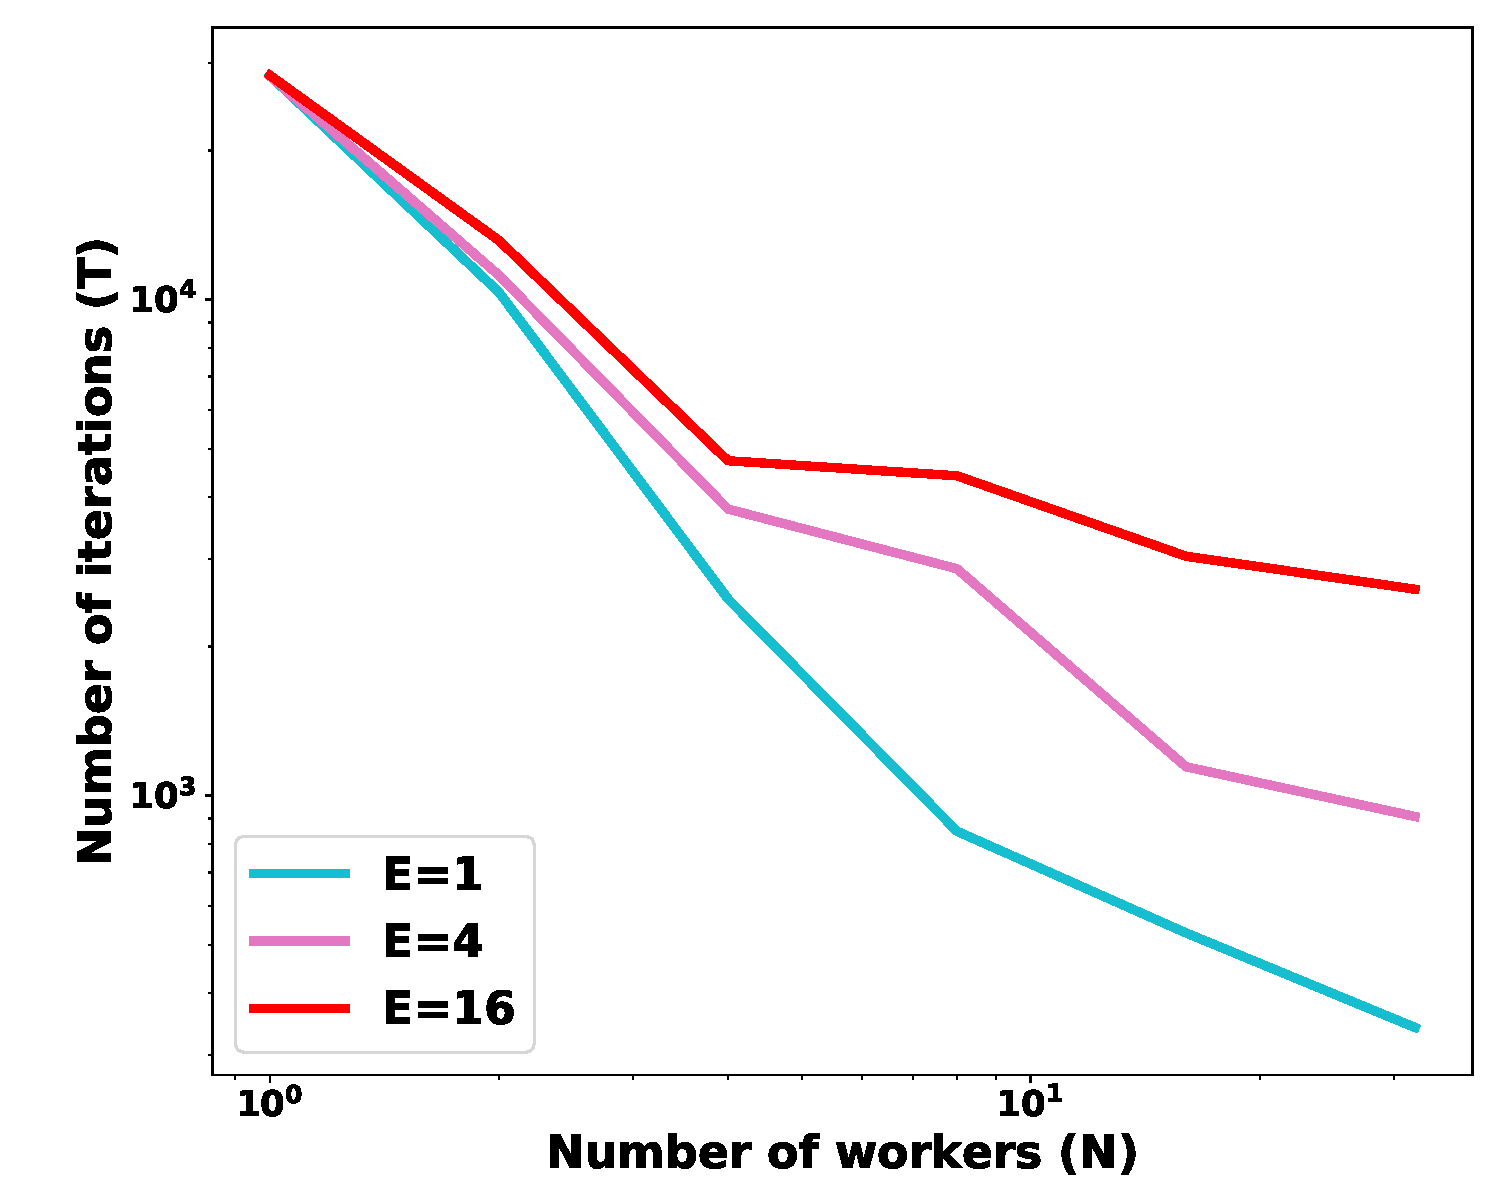
\includegraphics[width=0.33\textwidth]{fig/paper-nesterovspeedupNodesT-min-w8a-epsilon0131-reg1e-05.pdf} & 
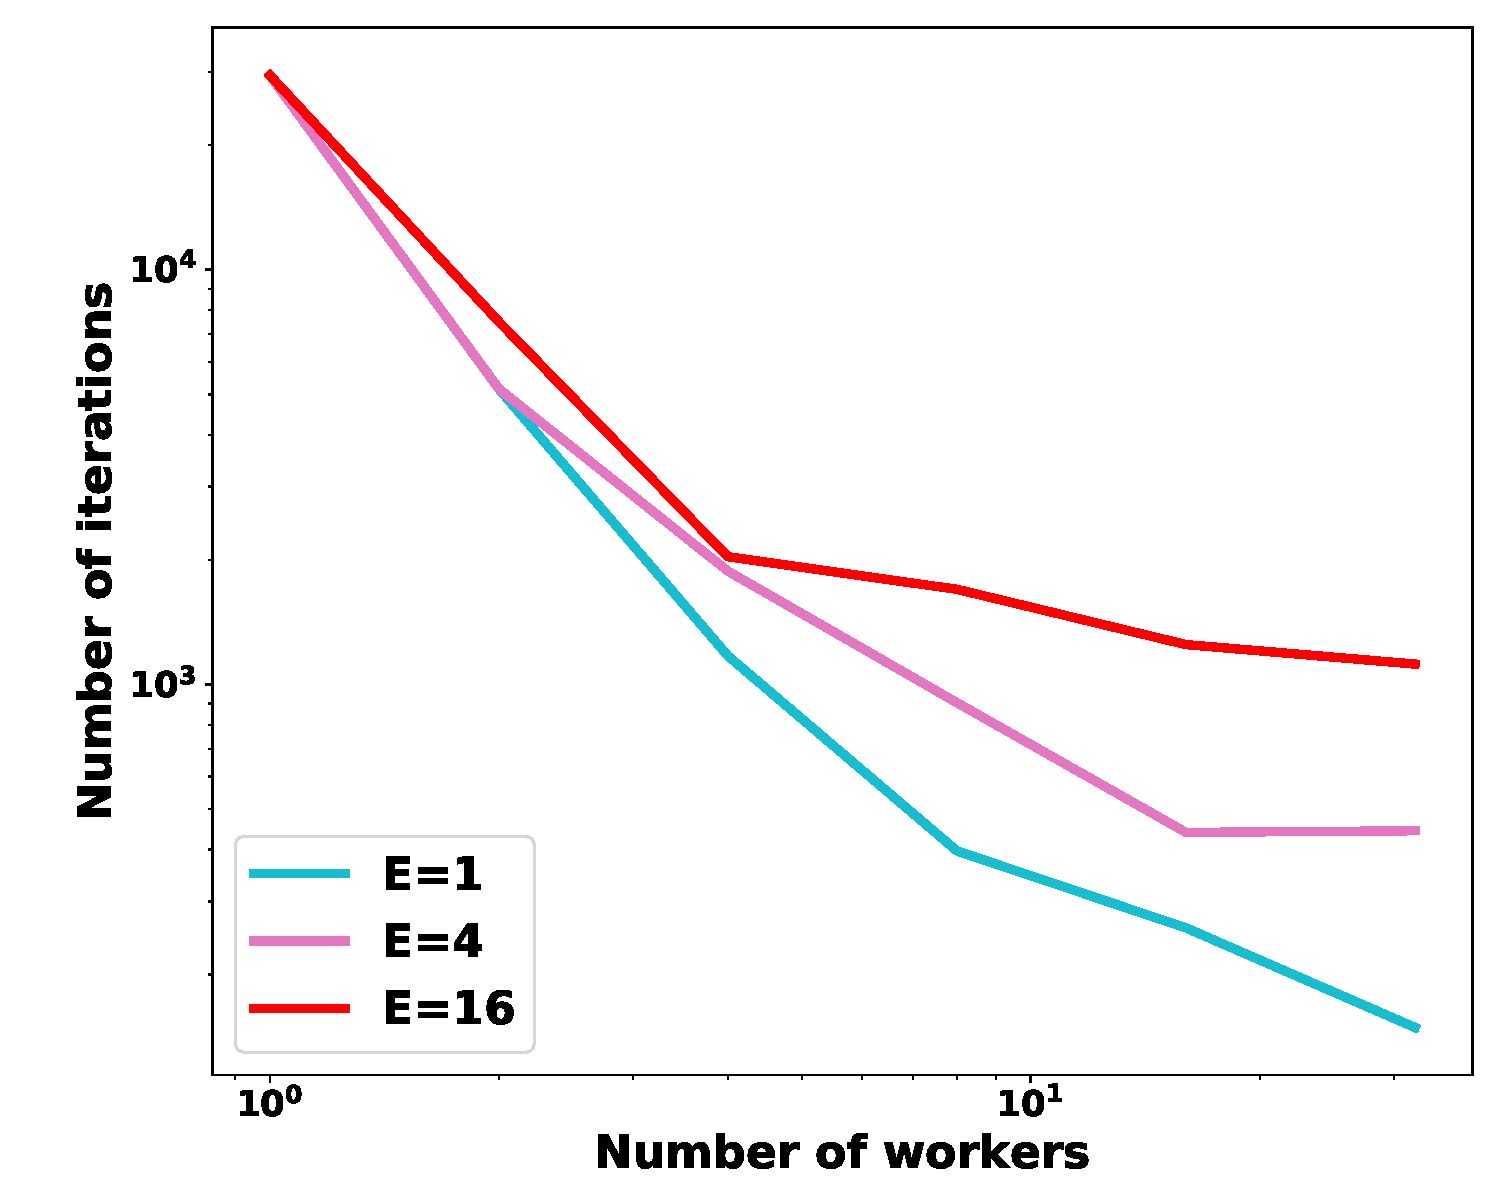
\includegraphics[width=0.33\textwidth]{fig/paper-nesterovspeedupNodesT-min-w8a-epsilon0134-reg0.pdf}
& 
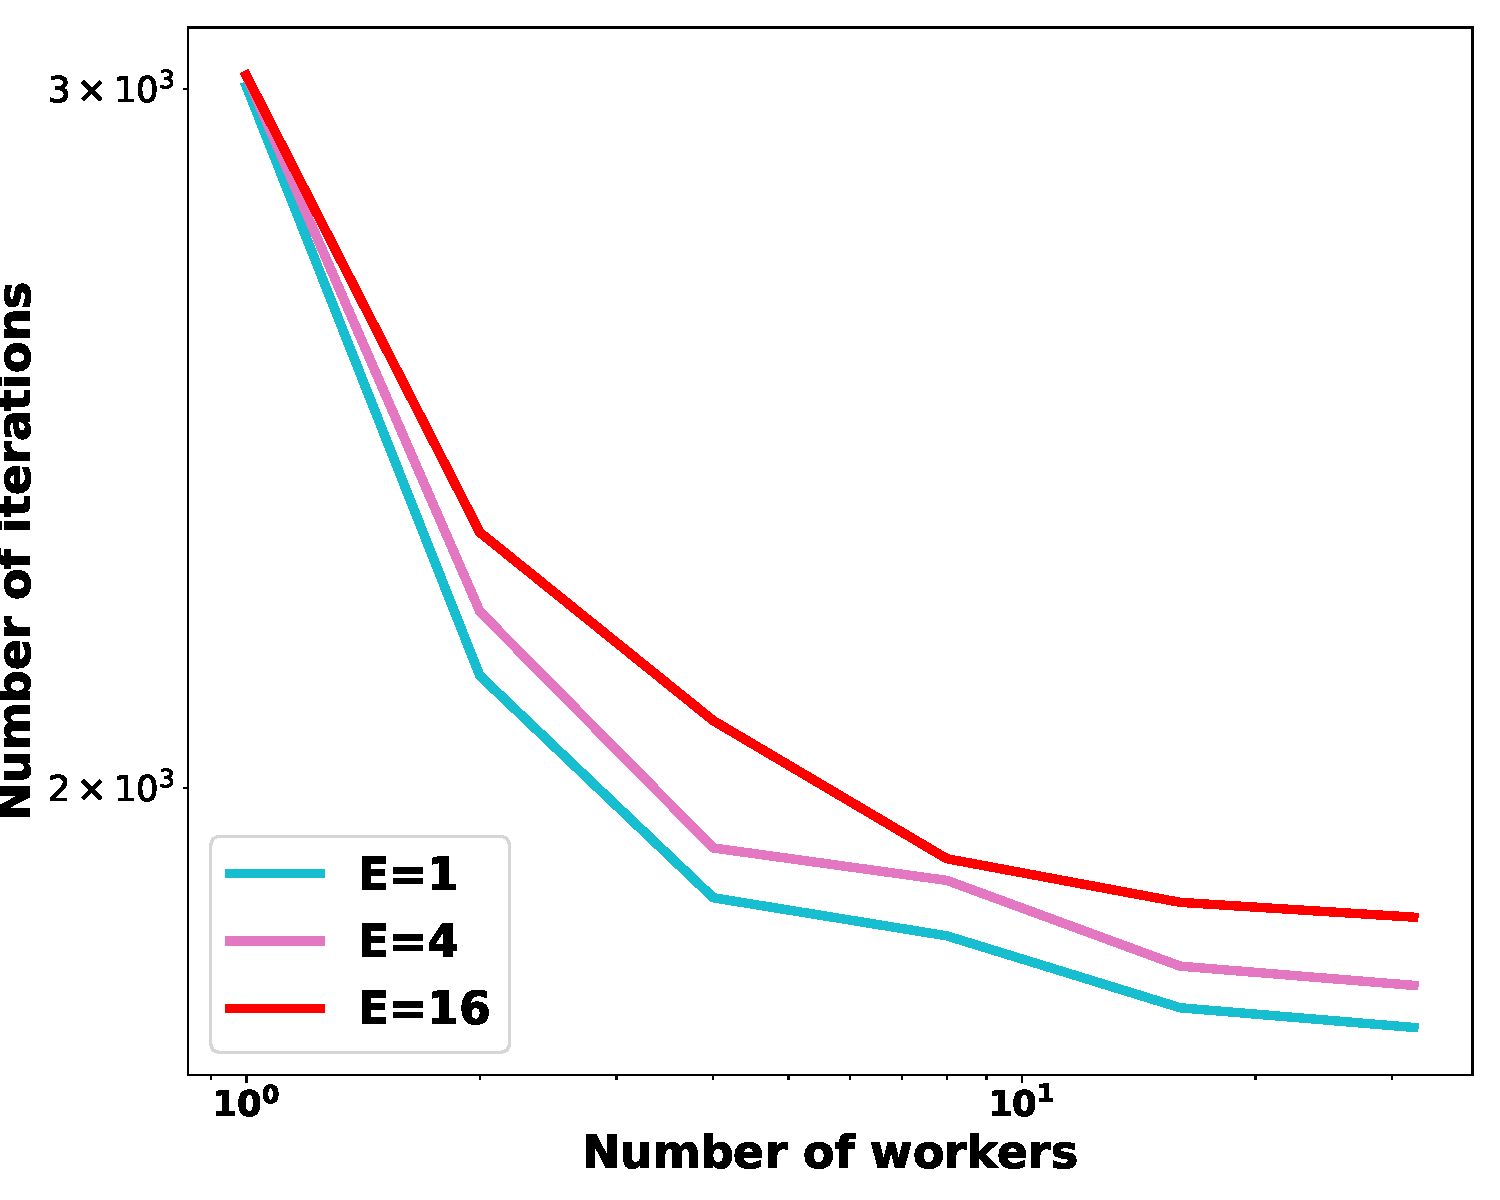
\includegraphics[width=0.33\textwidth]{fig/paper-lrnesterovspeedupNodesT-min-linearregressionw8a-epsilon002-reg0.pdf}\\
(a) Strongly convex objective & (b) Convex smooth objective & (c) Linear regression
	\end{tabular}
\caption{The linear speedup convergence of Nesterov accelerated FedAvg w.r.t the number of workers. }
\label{fig:nesterov}
\end{figure}


